\section{Hybrid PoW/PoS With Observers}
	\paragraph{}{
		It is widely accepted that the more people or entities dedicated to validating the state of the distributed ledger, the better and more secure the ledger and network will be. Researchers and developers continue to find approaches to increase network security and one of such explored approach is to enable mobile device owners to participate in the validation of the blockchain state. If this is achieved, it will greatly increase the security of a blockchain network by making attacks like 51\% difficult to achieve as the attacker will be competing with potentially millions of mobile devices dedicated to the network. 
	\vspace{-5mm}
	\paragraph{}{
	Unfortunately, the resource requirement for synchronizing, validating and storing chain state makes this approach costly and impractical for most mobile devices. 
Projects like Electroneum\cite{electroneum} perform simulations of mining that do not offer the network any improvement to secure other than to distribute the native coins to as many people as possible.	}

In the rest of this paper, I will describe a combination of hybrid PoW/PoS consensus with the inclusion of additional network participants known as Banknote scanners and validators, who implicitly act as chain observers while performing their roles in the creation of new coins. Banknote scanners tag the hash of a given block to a banknote and send these banknotes to the network for validation. The tagged banknotes are picked up by validators who manually verify the identity of the tagged block along with other defining features. The process of tagging and validating drives a system where banknotes providers and validators continuously vouch for blocks, thus, increasing block score and consequently the entire score of a branch. We believe this system will provide additional security and foster a more inclusive network where millions of people around the world can participate without much barrier. 
}

\vspace{5mm}
\subsection{Network Participants}

\begin{figure}[H]
  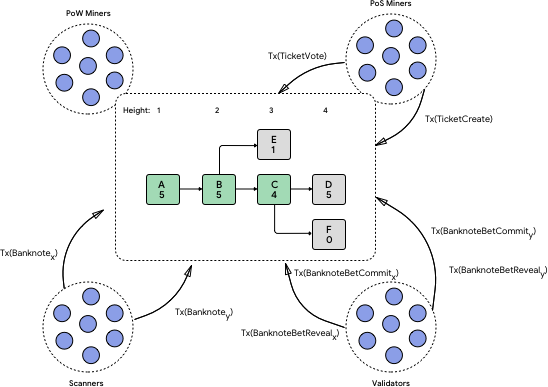
\includegraphics[width=\linewidth]{images/fig1}
  \caption{Network Participants}
  \label{fig:netpat}
\end{figure}
\vspace{3mm}

\paragraph{}{
Figure \ref{fig:netpat} describes a network of 4 participants namely Proof-of-Work miners, Proof-of-Stake miners, Banknote Scanners and Banknote validators. PoW miners are responsible for proposing new blocks. PoS miners endorse proposed blocks by voting for blocks they have confirmed to be valid under the consensus rule they follow. Banknote scanners provide the resource that is required to generate new coins which is used to incentivise other participants. This resource is a national banknote; an asset that is valuable and requires work to acquire. Banknote scanners provide this asset to the network in attempts to exchange for new coins after it undergoes and passes validations. Banknote validators are responsible for validating the correctness of a banknote. They do this by manually verifying attributes of the banknote and betting on the outcome of their validation. 
}


\subsection{Miners (PoW \& PoS)} 
\paragraph{}Proof-of-Work and Proof-of-Stake participants are classified as Miners. These are people or organizations who provide hardware and compute capabilities and form the network of computers that make up the system. They can also act as validators, endorsing blocks produced through Proof-of-Work processes. Miners in Bitcoin and other PoW systems earn reward for solving a computationally hard problem after which they broadcast a block containing the solution and a transaction that allocates their reward to the rest of the network. This system encourages competition between participants and forces them to seek more powerful and expensive mining equipments in hopes of outcompeting other miners. While this leads to an increased overall mining hash rate and network security, the wealth generated will be distributed unevenly, thus, creating a system that is centralized and reserved for the wealthy individuals and organizations. 

With PeopleMint, miners do not have monopoly over network reward as the resources that is used to produce rewards are provided by a different class of network participants who scan and validate banknotes. Contrary to the norm in Bitcoin-like systems where the miner rewards themselves, miners must collect banknotes up to a maximum amount before their blocks are accepted by the rest of the network and the resulting block reward shared between them and any other participants.  Without the other participants, creating and validating banknotes, a miner cannot generate new coins and any reward will be through transaction fees. 

\newpage
\subsection{Banknote Scanners}
\paragraph{}Banknote scanners are people who send images of national banknotes to be processed, included in blocks and generate new coins. As described in figure \ref{fig:netpat}, they send \textbf{\textit{TxBanknote}} transaction which contains a banknote that is tagged with the last 12 characters of the current tip block. There are millions of people across the world who have access to currency notes that may be supported and have never been processed by the Ellcrys network. These people can provide the system with this resource and become an essential category of users who work to ensure security by providing the supply of currency notes that generates the incentives while also acting as observers by implicitly voting for a block and preventing miners from going against consensus rules by refusing to tag blocks created by untrusted miners. 

Scanners cannot re-scan banknotes that have been previously processed and indexed. The currency notes they provide, are passed through a scanning protocol that provides a deterministic, effort-driven scanning procedure that standardises the way banknotes are scanned and offers economic difficulties to make abuse costly.   


\subsection{Banknote Validators}

Banknote validators are participants who depend on the actions of banknote scanners to fulfil their obligations to the network. Their primary activity is to fetch banknotes, endorse and predict the validity of the notes. There are two stages of validation:

\begin{description}
  \item[$\bullet$ Pre-Validation (a.k.a Vouching):] In this stage, validators (a.k.a Vouchers) verify and endorse banknotes that are in the transaction pool. They assert the correctness of the serial, denomination, currency code, tagged block hash and encode this information into a \textbf{\textit{TxVouch}} transaction. After $\rfrac{2}{3}$ of N required \textbf{\textit{TxVouch}} transactions are received for a banknote, Miner must create a \textbf{\textit{TxVouchedBanknote}} which includes the \textbf{\textit{TxBanknote}} transaction and the received \textbf{\textit{TxVouch}} transactions, broadcast it and add to the block they will mine.

  \newpage
  \item[$\bullet$ Pre-Validation Using Machine Learning (Alternative):] An alternative to the user-driven pre-validation stage is the use of machine learning to detect banknote details. The use of Machine Learning to aid validation has the advantage of automating the validation process, eliminating the need for vouchers and the incentives they need to function. However, supporting more banknotes will require more time and resources. 
  
   \item[$\bullet$ Validation:] After the \textbf{\textit{TxBanknote}} is added to a block, the final validation begins. Similar to the pre-validation stage, the validator (a.k.a bettor) verifies the correctness of serial, denomination, currency code, tagged block hash and endorses it by sending  \textbf{\textit{TxBanknoteBetCommit}} transaction containing the details in an encrypted form and subsequently a \textbf{\textit{TxBanknoteBetReveal}} transaction to reveal the votes for collation and reward disbursement.
 \end{description}
 
 During these stages, the validators are required to stake some amount of coins on every vouch or vote they make on a banknote as a "\textit{proof of truth}" which will be returned to them if they rightly predict the validity in the direction of the majority.  Bettors who failed to predict in the course of the majority lose their stake to the winning majority.  
 
 The purpose of the pre-validation phase is to identify the banknote, collect necessary information and confirm that required properties are in place. Validators help provide information that is used to construct a fingerprint for a given note. It is similar to a Captcha we all know and hate except this comes with network incentives. 
 
The validation stage randomly selects N number of \textbf{\textit{TxBanknoteBetReveal}} to reduce the ability of attackers to create fake identities, coordinate and vote for their notes. At the pre-validation stage, it is possible for the note owners to generate Sybil identities to vouch for their banknotes, but they will be unable to do so when the banknote is already in a block and ready to be voted on in the main validation phase since votes will be selected randomly. 

\section{Scanning}

\paragraph{}In this section, We will discuss the procedure and rules that should be followed by scanners to produce a valid digital representation of a banknote that can be processed and validated initially by miners and finally by banknote validators/bettors.



\subsection{Introduction}

\paragraph{}The scanning protocol dictates a set of steps to be carried out by people who intend to exchange banknotes for the native coin. These banknotes act as raw materials for creating new coins, providing the block rewards shared between the block creator, block endorsers, validators/bettors and any other future network participants. Without the introduction of new banknotes into the system, new coins are not created, and the network will be unable to incentivize participants. People around the world send currency notes and hope that validators find their submission acceptable. However, naively asking people to send still images exposes the network to the following attacks:


\subsection{Counterfeit \& Image Manipulation}
\label{sec:counterfeit_man}
The most obvious problem is the issue of counterfeit. The likelihood of people feeding the network with banknotes that have been counterfeited or manipulated using image editing software is high. Manipulation using image editing tools is cheap; The attacker only needs to change the serial of one banknote many times. However, the process of counterfeiting currency notes is not cheap or a zero cost operation. We believe that with the right scanning and economic model, we will be able to replicate the cost constraints that existing counterfeiting enterprises face and make it costly for them to move their business to the Ellcrys network. We have identified some of the cost factors experienced by these organisations and way by which we can replicate them:

\vspace{1mm}
\begin{description}
  \item[$\bullet$ Physical Cost:] Counterfeiters are in the business of creating fake currencies in their physical, tangible form. They invest in infrastructure that enables them to reach their goals. Their expenditure includes rent, raw materials, vehicles, printers, electricity and other equipment. Like manufacturing business, they incur production costs.   
  
   \item[$\bullet$ Transportation Cost:] After the production of counterfeited currencies, the counterfeiters move them from their hidden location to the distributor,  the end-users and other people in the supply chain. Transporting this product is very risky to them and comes at a cost. 
   
   \item[$\bullet$ Workforce:] Counterfeiters employ labourers who possess varying skill sets that are required to produce quality counterfeits. They include but not limited to designers, printers, cutters to artists. These people receive monetary payments for the services they render.
   
   \item[$\bullet$ Competition:] They also contend with their competitors concerning the quality of the product they distribute. Like regular, legal businesses, they will be willing to spend on improving the quality of their product to guarantee their ability to compete, retain and acquire new customers. 
   
   \item[$\bullet$ Time:] Producing quality counterfeit notes takes a lot of care and time. The process is so delicate that every detail of a real currency must be carefully and skillfully replicated. The more time expended, the more the risk and financial requirement. 
   
   \item[$\bullet$ Uncertainty:] Regardless of all the care and financial investment put into the production of fake currencies; Counterfeiters and people in this line of work are never always guaranteed a return on their investment. Their distribution pipeline may be unexpected compromised. Their production location could are raided at any time. One or two employers might be arrested or just become unavailable.    
   
 \end{description}

\paragraph{}{
	As described above, even counterfeiters incur some cost that makes the production of counterfeit currency notes costly in a similar way the acquisition of an original banknote by ordinary users requires cost which is the expense of energy or the offering of skill to a person, employer or organisation. Nobody should be able to receive the native coin without giving something of value. The scanning protocol must make sure that the cost factors described above are in place to a reasonable extent. 
}

\subsection{Replicating Cost Factors}

In this section, We discuss ways to replicate the cost factors described in  \autoref{sec:counterfeit_man} ins such a way that will provide have similar difficulties built into the protocol. 

\vspace{1mm}
\subsubsection{Physical Cost}
\label{sec:physical_cost}
 To support physical cost, we must be able to force the use of material-based, tangible currency notes as opposed to static versions of a currency that may have been created or modified in an image editing software. If the tangibility proof is made mandatory, then it will be costly to set up farms dedicated to mass producing or scanning banknotes. These are the proposed methods to enforce tangibility:
 
 \vspace{1mm}
\begin{description}
  \item[$\bullet$ Fixed-Length Video Format:] The first step is to require banknotes to be sent to the network encoded in a fixed-length video format. It is more difficult to cleanly and unnoticeably modify a video than it is to alter a still image.
  
  \item[$\bullet$ Hashstamping:] The video scanning procedure must integrate a mechanism that requires work to be carried out as "proof of work" mechanism. We propose that scanners must flip the front and back of the banknote and proceed to write the last 12 characters of the hash of the most recent block on the note using a pencil or any other writing tool that does not permanently deface the banknote. The scanning ritual must be done within a fixed amount of time (e.g. 15 seconds). Writing the last 12 characters of a recent block's hash servers to (1) Force the video to expire after a number of blocks have been confirmed (2) Prevent stockpiling of videos create days ago (3) Used as an implicit means of voting for a block and consequently used to decide the value of a branch over another (fork choice algorithm). 
   
 \end{description}
 
 

\vspace{1mm}
\subsubsection{Transportation Cost}
\paragraph{}Counterfeiters will continue to incur the transportation cost of moving materials used to create fake banknotes because they will continue to distribute their counterfeit notes to maximise their profit. Also, they will also pay network transaction fees to transfer the banknotes to the network like regular users. There will be competition between them and other scanners. They are more likely to increase transaction fees to gain more priority over other scanners. Measures must be put in place to prevent an unfair fee market by normalising scanning fees such that good scanners are not edged out due to their inability to pay higher transaction fees. 


\vspace{1mm}
\subsubsection{Workforce Cost}
\paragraph{}Counterfeiters and people who may create farms dedicated to scanning banknotes will need to invest more into their operations to accommodate more human scanners and will require more space if they need to increase capacity, thus, further re-enforcing the physical cost of scanning mentioned in \autoref{sec:physical_cost}. 


\vspace{1mm}
\subsubsection{Competition Cost}
\paragraph{}The fact that the network is open to millions of people around the world with very little or no barrier, counterfeiters and scanning farms may find that they are unable to outcompete conventional scanners. The normalisation of fees will also work to create a levelled network. Counterfeiters may prefer to continue with their original business model. 



\vspace{1mm}
\subsubsection{Time \& Uncertainty Cost}
\paragraph{}Counterfeiters will not instantly get coins successfully exchanged for an excellently produced banknote. Blockchain networks typically require rewards to reach a certain maturity period before they are spendable. During this time, the coin may gain or lose value. If there is a loss of coin value, the counterfeiter may have spent more to produce the banknotes that resulted in the low-value reward. Furthermore, they are subjected to scrutiny by the validators whom they are unable to control and may have their scanned notes rejected.  


\vspace{1mm}
\subsection{Stockpiling}
Stockpiling is the act of collecting and storing a pre-scanned banknote to be exchanged at a later date, possibly at a time when the price of the coin is high. People who stockpile many notes may have the ability to plan and significantly affect the market and economics of the network within a short time and at little cost to them. By tagging each banknote with the last 12 characters of a new block's hash, We force pre-scanned banknotes to expire after a fixed number of block confirmations (e.g. After six blocks starting from the tagged block).  This process is called \textbf{"hashstamping"}


\newpage
\subsection{Selection Bias}
Selection bias describes a situation where scanners begin to centralise towards a single or small sets of banknotes that they believe will have a better network exchange rate; Network exchange rate determines how much Ellies are exchangeable for a currency note. The number of ELL exchanged for USD banknote will be different from that of EUR. Additionally, miners may also begin to censor banknotes that do not fall within a given set of banknote types that have certain qualities. If this is allowed to happen, then scanners in countries with low-valued banknotes will be practically disenfranchised. 

An approach to solving this is to deny miners and banknote validators the ability to select banknotes. The protocol should randomly select a set of notes that are eligible for scanning during a given epoch. Random selection of currency type forces scanners and validators to work within the selected choices.  It also provides a property that encourages scarcity and alternates coin generation between regions/countries. If professional scanning becomes an occupation, people would have to acquire banknotes from a different region to be able to participant in coin generation.  


\section{Banknote Selection}

In this section, We will describe the selection procedure employed by miners for selecting banknotes. It is important for this selection process to promote the following properties:
 \vspace{1mm}
\begin{description}
  \item[$\bullet$ Censorship-Resistance:] This requires everyone to have a fair chance to exchange their banknotes for the native coin. If scanners and miners can decide what notes are worth processing/validating, then thousands across the world will be unfairly denied the chance to participate. 
  \item[$\bullet$ Liveness:]  Liveness means the network continues to progress even when blocks do not contain banknotes. In such a case, miners will have to rely only on fees as their reward since block generation does not result in the creation of new coins.
  \item[$\bullet$ Scarcity:] Excessive creation of new coins will significantly reduce the value of existing coins in circulation. We must provide constraints to reduces inflation to the existing monetary base. 
  
\end{description}

\begin{figure}[H]
  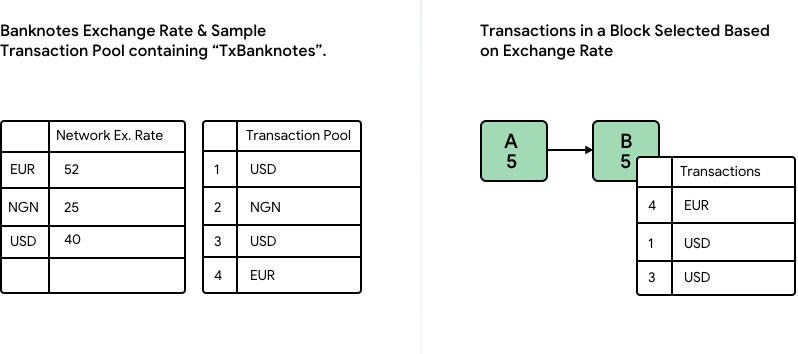
\includegraphics[width=\linewidth]{images/fig2}
  \caption{Selection Bias: Banknotes of higher exchange value are preferred}
  \label{fig:select_bias}
\end{figure}
\vspace{3mm}


\paragraph{} On the left of Fig \ref{fig:select_bias}, We are presented with a set of \textbf{\textit{TxBanknote}} transactions in a transaction pool and their ELL exchange rate. On the right, We show transactions that were selected and included in a block \textbf{B}. Due to the difference in the real-world value of currencies, miners are incentive to select only transactions that will result in higher revenue. In the illustration, these currencies are \textbf{EUR} and \textbf{USD}. Lower-valued currencies will only be considered when a coin reward limit is introduced, and only lower-valued banknotes are sufficient to reach the limit without exceeding it. 

\subsection{Random Banknote Selection}
Miners follow an unpredictable but deterministic algorithm to select N currency types that can be accepted and processed in blocks created over a given epoch. They use the hash of the current block to seed a pseudo-random number generator and subsequently fetch more banknote types by extending the seed with the byte equivalent of the last selected currency type id. Figure \ref{fig:select_algo} describes the selection algorithm in Go programming language. 
The process is repeated at the beginning of a new epoch. 

\subsubsection{Benefits of Random Banknote Selection}
These are some of the benefits of derived from selecting banknotes types randomly. 
\vspace{1mm}
\begin{description}
  \item[$\bullet$] The Miners, Scanners and Validators ability to censor banknotes transactions based on exchange rate value is reduced as they have no control over what sets of banknotes are valid per epoch.
  \item[$\bullet$] Fair opportunity for citizens within the jurisdictions of the selected currency types to exchange their notes. 
  \item[$\bullet$] Makes banknote stockpiling much more difficult as scanners are unable to predict which banknotes will be eligible.
  \item[$\bullet$] Regulation of scanners population; The number of people able to scan will be randomly regulated. 
  
\end{description}

\begin{figure}[H]
  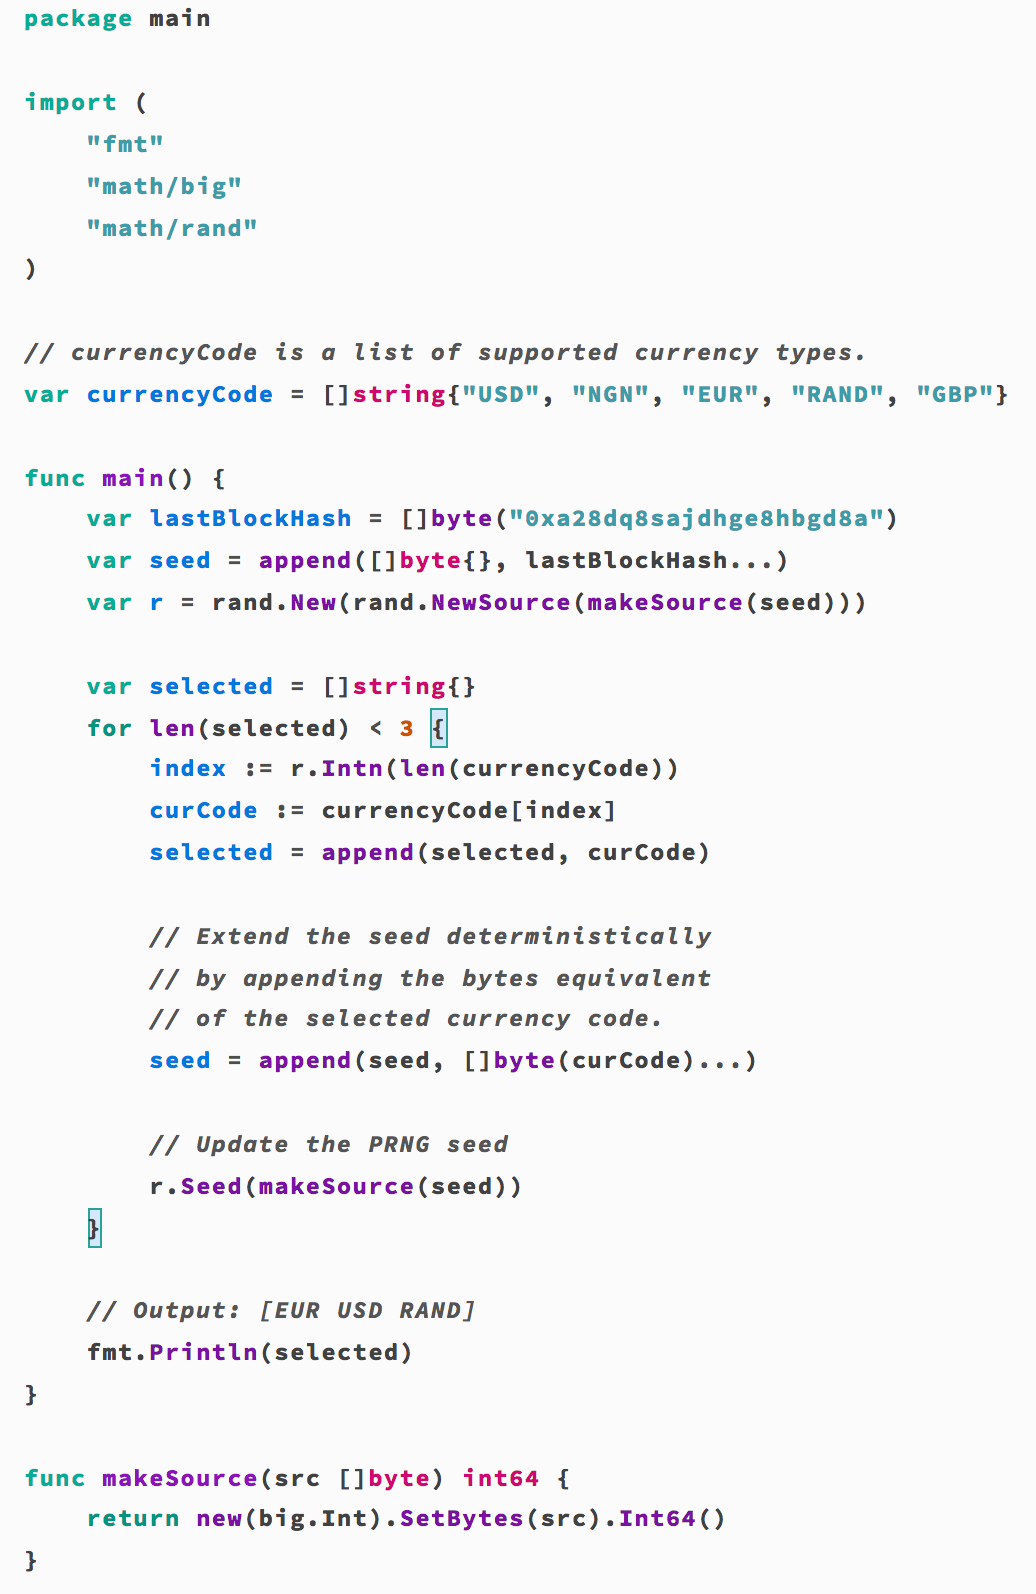
\includegraphics[width=\linewidth]{images/fig3}
  \caption{Random Selection Algorithm}
  \label{fig:select_algo}
\end{figure}
\vspace{3mm}


\section{Network Exchange Rate}

The network exchange rate determines how much native coin is exchangeable for a given banknote type. For instance, how much will ELL be exchanged for 1 USD? This information will typically be hardcoded into the client allowing all nodes to perform same exchange calculations. Similar to Bitcoin, We can reduce exchange rates over time to produce the same effect of halving rewards over time. 




\section{Conclusion}

This paper introduced a mining protocol that can be used to create a more equitable reward system for a distributed system. However, it is incomplete as there is a need for further study, particularly on incentives alignment and security. We are actively looking at this issues and will release updated versions of these document in the future. 





















 
